% 12 variables in here:
% H_1 = 10.0, H_2 = 10.0, H_3 = 10.0, U_1 = 0.0, U_2 = 0.0, U_3 = 0.0, h_1 = 9.0, h_2 = 10.0, h_3 = 10.0, u_1 = 0.0, u_2 = 0.0, u_3 = 0.0
\begin{figure}[h!]
\centering
  % \subfigure[] {
  %   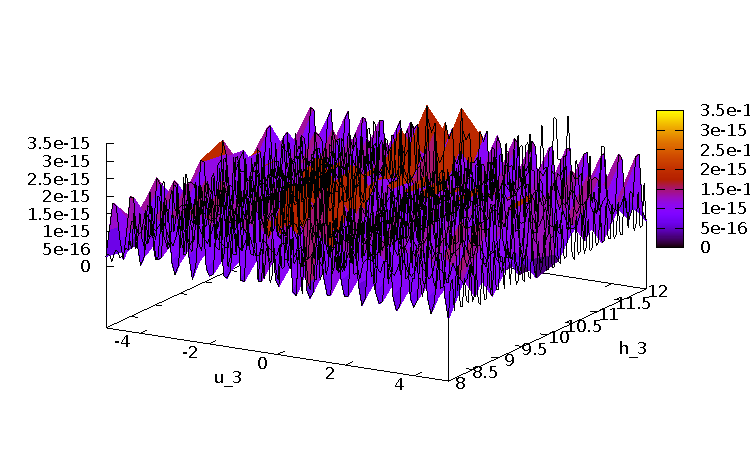
\includegraphics[scale=\zoomfactor]{{{equidist_3_alles_default_ausser_p1_9_0/10.0_10.0_10.0_0.0_0.0_0.0_9.0_10.0_y_0.0_0.0_xf00}}}
  % }
  \subfigure[Impulse error for $p_2^L$] {
    \begin{tikzpicture}
      \node at (0,0) {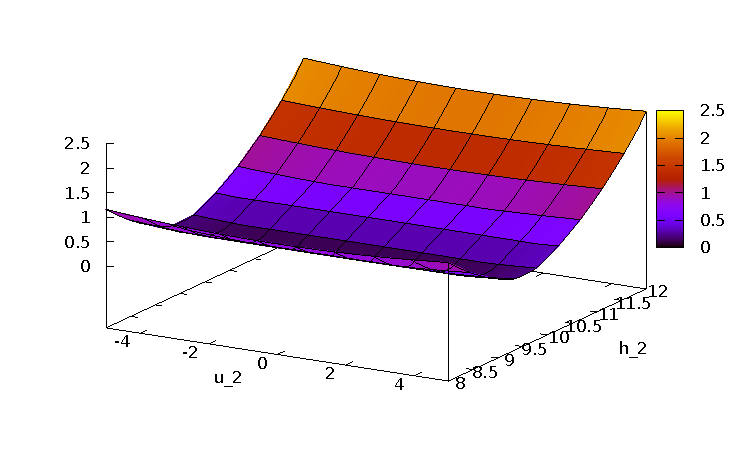
\includegraphics[scale=\zoomfactor]{{{equidist_3_alles_default_ausser_p1_9_0/10.0_10.0_10.0_0.0_0.0_0.0_9.0_y_10.0_0.0_x_0.0f01}}}};
      \node[align=right, text width=3cm] at (.2,1.33) {\textsf{\tiny{Impulse error}}};
      \draw(1.8,1.34) -- +(.4cm,0);
    \end{tikzpicture}
  }
  \subfigure[Impulse error for $p_3^L$] {
    \begin{tikzpicture}
      \node at (0,0) {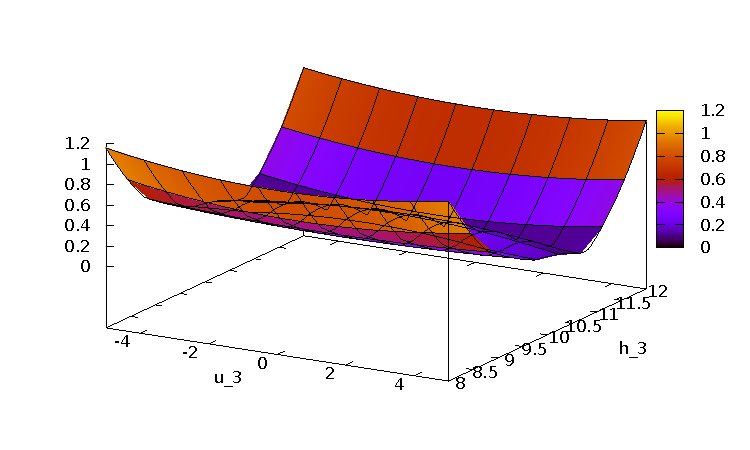
\includegraphics[scale=\zoomfactor]{{{equidist_3_alles_default_ausser_p1_9_0/10.0_10.0_10.0_0.0_0.0_0.0_9.0_10.0_y_0.0_0.0_xf01}}}};
      \node[align=right, text width=3cm] at (.2,1.33) {\textsf{\tiny{Impulse error}}};
      \draw(1.8,1.34) -- +(.4cm,0);
    \end{tikzpicture}
  }
  % \subfigure[] {
  %   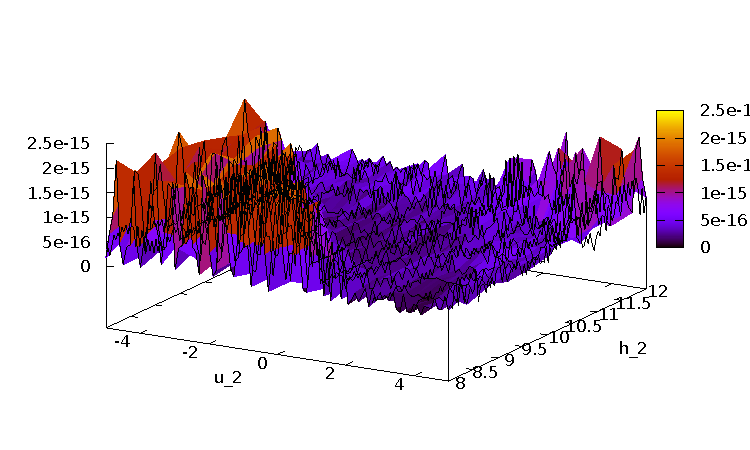
\includegraphics[scale=\zoomfactor]{{{equidist_3_alles_default_ausser_p1_9_0/10.0_10.0_10.0_0.0_0.0_0.0_9.0_y_10.0_0.0_x_0.0f00}}}
  % }
  % \subfigure[] {
  %   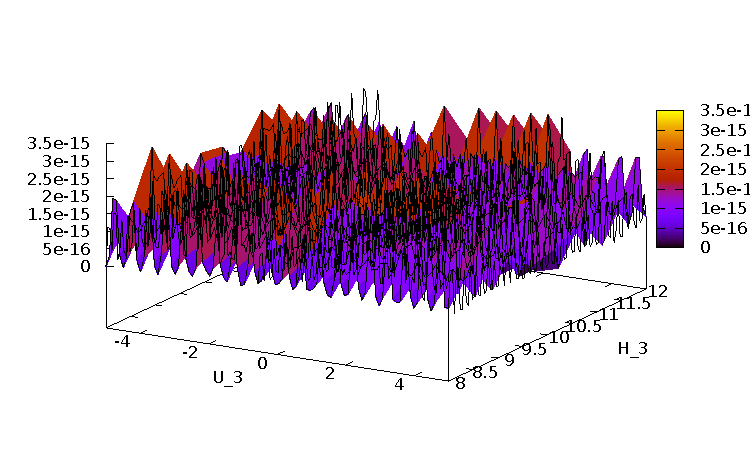
\includegraphics[scale=\zoomfactor]{{{equidist_3_alles_default_ausser_p1_9_0/10.0_10.0_y_0.0_0.0_x_9.0_10.0_10.0_0.0_0.0_0.0f00}}}
  % }
  % \subfigure[Impulse error for $p_1^R$] {
  %   \begin{tikzpicture}
  %     \node at (0,0) {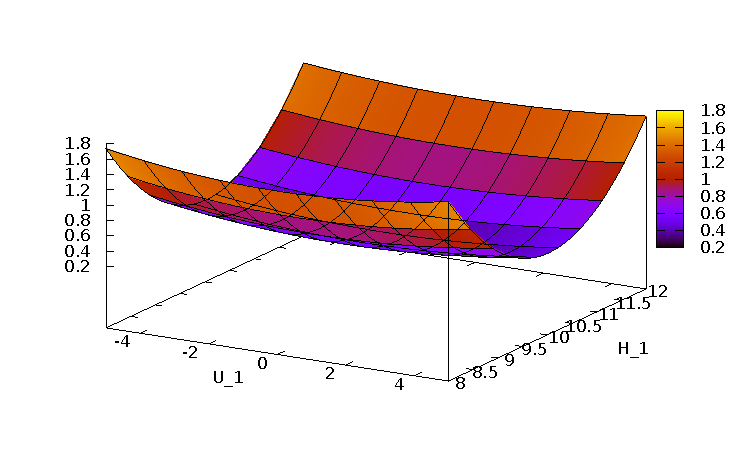
\includegraphics[scale=\zoomfactor]{{{equidist_3_alles_default_ausser_p1_9_0/y_10.0_10.0_x_0.0_0.0_9.0_10.0_10.0_0.0_0.0_0.0f01}}}};
  %     \node[align=right, text width=3cm] at (.2,1.33) {\textsf{\tiny{Impulse error}}};
  %     \draw(1.8,1.34) -- +(.4cm,0);
  %   \end{tikzpicture}
  % }
  % % \subfigure[] {
  % %   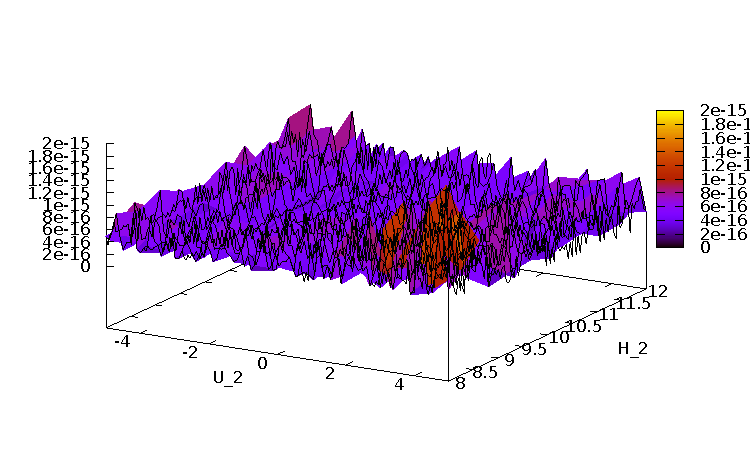
\includegraphics[scale=\zoomfactor]{{{equidist_3_alles_default_ausser_p1_9_0/10.0_y_10.0_0.0_x_0.0_9.0_10.0_10.0_0.0_0.0_0.0f00}}}
  % % }
  % \subfigure[Impulse error for $p_2^R$] {
  %   \begin{tikzpicture}
  %     \node at (0,0) {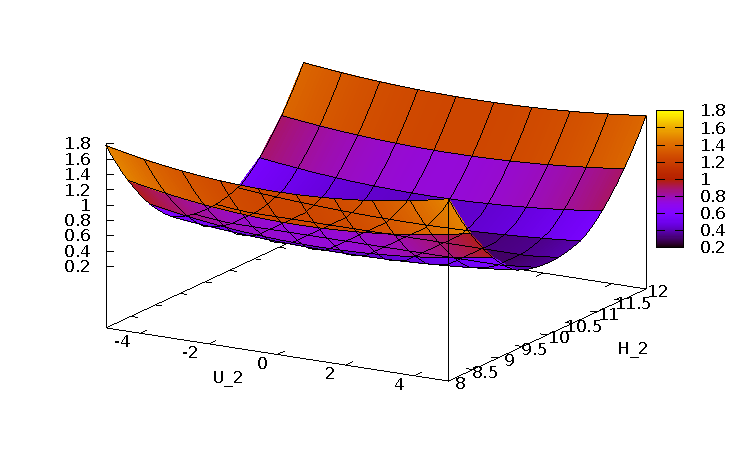
\includegraphics[scale=\zoomfactor]{{{equidist_3_alles_default_ausser_p1_9_0/10.0_y_10.0_0.0_x_0.0_9.0_10.0_10.0_0.0_0.0_0.0f01}}}};
  %     \node[align=right, text width=3cm] at (.2,1.33) {\textsf{\tiny{Impulse error}}};
  %     \draw(1.8,1.34) -- +(.4cm,0);
  %   \end{tikzpicture}
  % }
  % \subfigure[Impulse error for $p_3^R$] {
  %   \begin{tikzpicture}
  %     \node at (0,0) {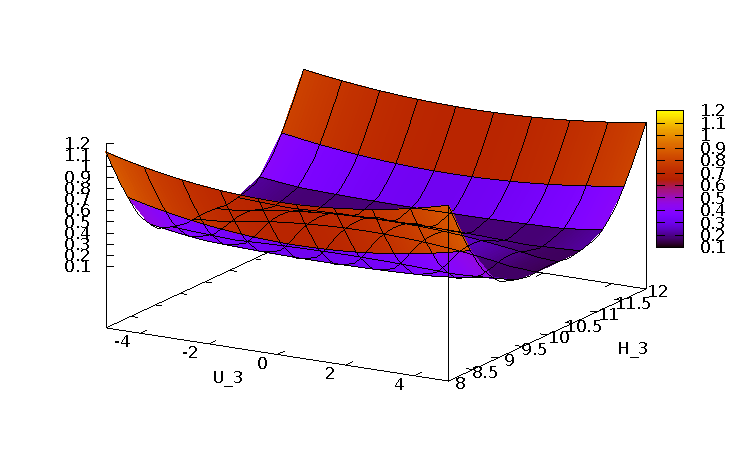
\includegraphics[scale=\zoomfactor]{{{equidist_3_alles_default_ausser_p1_9_0/10.0_10.0_y_0.0_0.0_x_9.0_10.0_10.0_0.0_0.0_0.0f01}}}};
  %     \node[align=right, text width=3cm] at (.2,1.33) {\textsf{\tiny{Impulse error}}};
  %     \draw(1.8,1.34) -- +(.4cm,0);
  %   \end{tikzpicture}
  % }
  % \subfigure[] {
  %   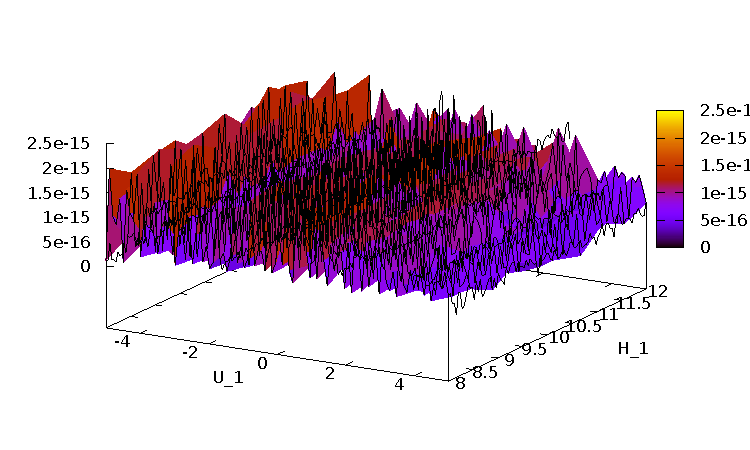
\includegraphics[scale=\zoomfactor]{{{equidist_3_alles_default_ausser_p1_9_0/y_10.0_10.0_x_0.0_0.0_9.0_10.0_10.0_0.0_0.0_0.0f00}}}
  % }
\caption{Impulse errors for suport points at $\{0, \frac{1}{2}, 1\}$. The point $p_1^L=(9,0)$, all other points are $(10,0)$. The plots look very similar in shape to the corresponding plots in figure \ref{fig:three-points-h1-} (where we used support points from Gaussian quadrature), but the errors are larger compared to them.}
\label{fig:equidist_3_alles_default_ausser_p1_9_0}
\end{figure}

%%% Local Variables:
%%% TeX-master: "../results.tex"
%%% End:
